%iffalse
\let\negmedspace\undefined
\let\negthickspace\undefined
\documentclass[journal,12pt,onecolumn]{IEEEtran}
\usepackage{cite}
\usepackage{amsmath,amssymb,amsfonts,amsthm}
\usepackage{graphicx}
\usepackage{textcomp}
\usepackage{xcolor}
\usepackage{hyperref}
\usepackage{mathtools}
\usepackage{gensymb}
\usepackage{tkz-euclide} 
\newcommand{\myvec}[1]{\begin{pmatrix} #1 \end{pmatrix}}
\newcommand{\brak}[1]{\left( #1 \right)}

\begin{document}
\bibliographystyle{IEEEtran}

\vspace{3cm}
\title{1-1.6-29}
\author{AI24BTECH11013-Geetha Charani}
\maketitle
\bigskip

\renewcommand{\thefigure}{\theenumi}
\renewcommand{\thetable}{\theenumi}

\begin{enumerate}
    \item Show that the points \( A\brak{2, 3, -4}, B\brak{1, -2, 3}, \) and \( C\brak{3, 8, -11} \) are collinear.\\
    
    \textbf{Solution:} Given,\\
    $
    A = \myvec{2 \\ 3\\ -4}, B = \myvec{1 \\ -2 \\ 3}, C = \myvec{3 \\ 8 \\ -11}
    $
    
    For points $ A, B, C $ to be collinear, the rank of the matrix formed by $ B - A $ and $ C - A $ must be less than 2.\\
    
    $
    \Vec{B} - \Vec{A} = \myvec{1 \\ -2 \\ 3} - \myvec{2 \\ 3 \\ -4} = \myvec{-1 \\ -5 \\ 7}
    $
    $
    \Vec{C} - \Vec{A} = \myvec{3 \\ 8 \\ -11} - \myvec{2 \\ 3 \\ -4} = \myvec{1 \\ 5 \\ -7}
    $
    
    Now, form the matrix $ M $ as:
    $
    M = \myvec{-1 & 1 \\ -5 & 5 \\ 7 & -7}
    $
    
		The rank of this matrix is 1, since the second column is a scalar multiple of the first. Therefore, the rank of the matrix is less than 2, which implies that the points are collinear.
\end{enumerate}

\begin{figure}[ht]
   \centering
   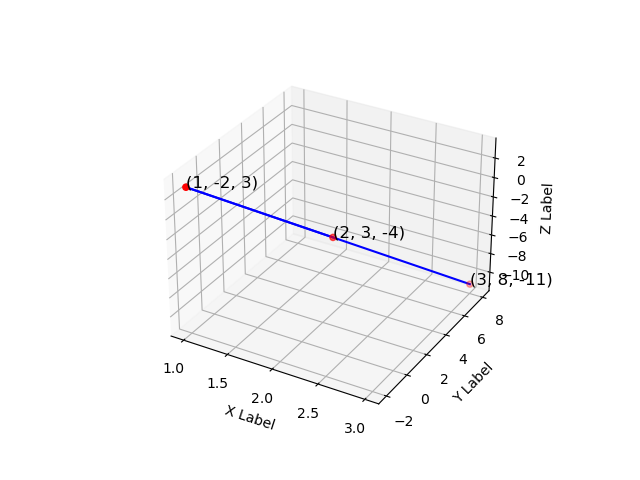
\includegraphics[width=0.7\linewidth]{figs/fig_1.png}
   \caption{Graph of Collinear Points}
   \label{q1}
\end{figure}

\end{document}

